\documentclass{article}
\usepackage{algorithm}
\usepackage{algpseudocodex}
\usepackage{graphicx}
\usepackage{amsmath}
\usepackage{xcolor}
\usepackage{listings}
\usepackage{hyperref}

\definecolor{codegreen}{rgb}{0,0.6,0}
\definecolor{codegray}{rgb}{0.5,0.5,0.5}
\definecolor{codepurple}{rgb}{0.58,0,0.82}
\definecolor{backcolour}{rgb}{0.95,0.95,0.92}

\lstdefinestyle{mystyle}{
    backgroundcolor=\color{backcolour},   
    commentstyle=\color{codegreen},
    keywordstyle=\color{magenta},
    numberstyle=\tiny\color{codegray},
    stringstyle=\color{codepurple},
    basicstyle=\ttfamily\footnotesize,
    breakatwhitespace=false,         
    breaklines=true,                 
    captionpos=b,                    
    keepspaces=true,                 
    numbers=left,                    
    numbersep=5pt,                  
    showspaces=false,                
    showstringspaces=false,
    showtabs=false,                  
    tabsize=2
}

\lstset{style=mystyle}

\title{CSEP590 : Applied Cryptography: Homework 5}
\author{Karuna Sagar Krishna}

\begin{document}
    \maketitle

    \section*{Task 1}
    The protocol described in this question is similar to the forward secure asymmetric AKE protocol 1 from the lectures. The difference is that the protocol in question doesn't sign the ephemeral public key (EPK) sent by the Bank to Alice. This allows for any man-in-the-middle (MITM) attacker to tamper with $EPK$.

    \begin{figure}[H]
        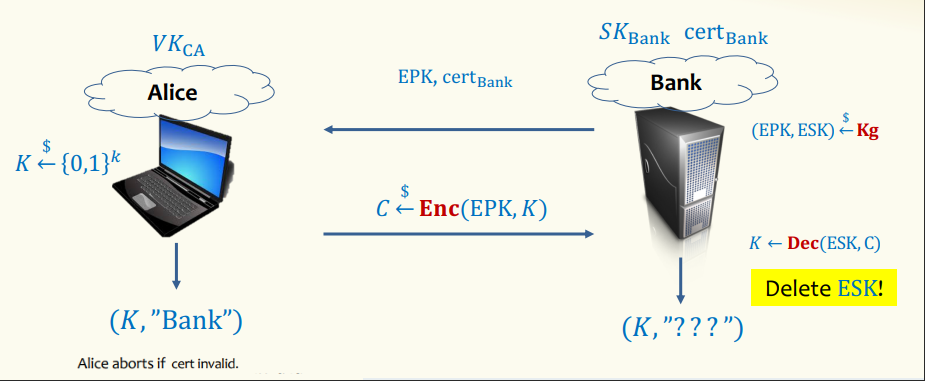
\includegraphics[width=1\textwidth]{protocol.png}
    \end{figure}

    So consider Eve (MITM) who generates her own $EPK'$ and $ESK'$. She intercepts the traffic between Bank and Alice as shown below. Eve sends $EPK'$ and $cert_{bank}$ to Alice. Alice verifies $cert_{bank}$ and finds that it is valid, generates a session key $K$, encrypts $K$ using $EPK'$ to generate $C'$ that is sent on the network. Since Eve knows $ESK'$, she can decrypt $C'$ and learn $K$. She then encrypts $K$ using $EPK$ to generate $C$ and sends to the bank. Essentially, Alice thinks she is talking to Bank but she is actually talking to Eve. Since Eve has learnt the session key $K$, she can decrypt all messages between Alice and Bank going forward.

    \begin{figure}[H]
        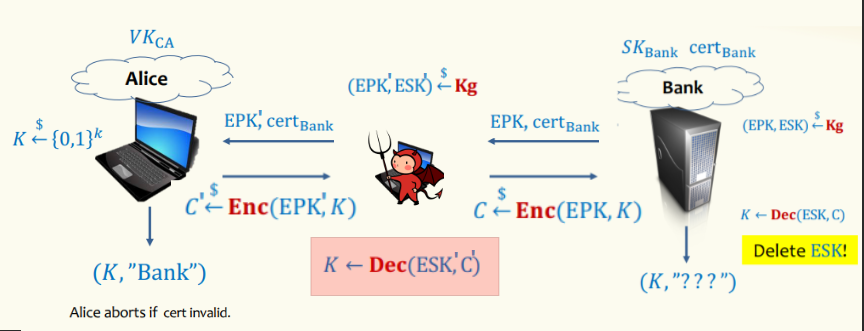
\includegraphics[width=1\textwidth]{mitmAttack.png}
    \end{figure}

    \section*{Task 2a}
    The protocol described in this question is similar to the symmetric AKE discussed in class. However, there are big differences in the way cipher text $C$ and signature $\sigma$ is calculated by Alice. Below is the pictorial representation of the protocol described in the question. Essentially, the identity of Alice and Bank are missing from the cipher text and signature respectively.

    \begin{figure}[H]
        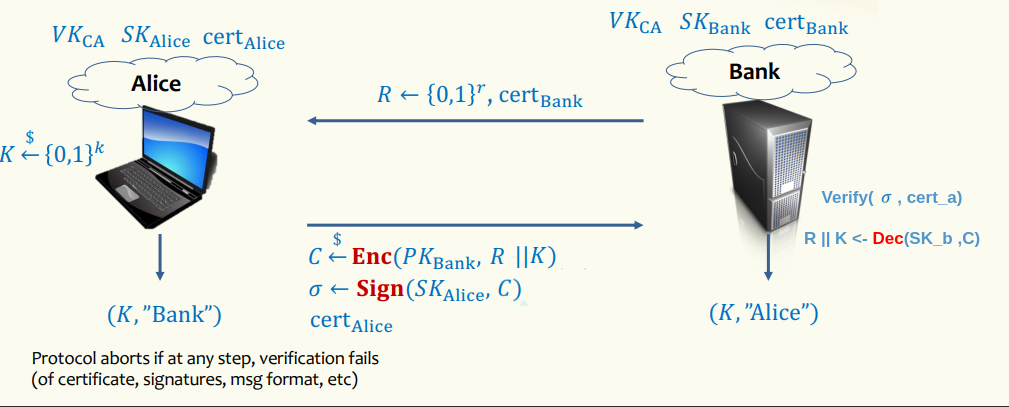
\includegraphics[width=1\textwidth]{protocol2.png}
    \end{figure}

    A MITM attacker can leverage the lack of identity if cipher text and signature and impersonate Alice as show below. Eve intercepts the traffic from Alice to Bank; she doesn't change the cipher text (assuming we are using IND-CCA secure encryption). However, she signs the cipher text using her secret key $SK_{Eve}$ and also sends her certificate $cert_{Eve}$ to Bank. Bank verifies the signature using the public key in the certificate. Though Eve tampered with the signature and certificate, Bank cannot tell identify this. Bank then decrypts the cipher text using its secret key $SK_{bank}$ to recover the session key $K$ and random nonce $R$. Since the cipher text was not tampered by Eve, the nonce verification passes. The bank can then output the session key $K$ and the identity as Eve since the certificate is the only place where the identity is present. Though Eve has not learnt the session key $K$, she has tricked the Bank into thinking that it is talking to Eve instead of Alice. This is essentially the "identity misbinding attack" described in the question.

    \begin{figure}[H]
        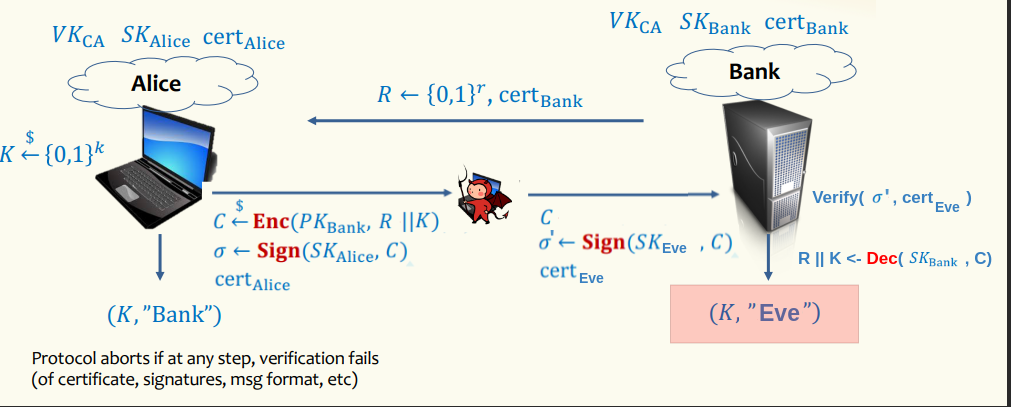
\includegraphics[width=1\textwidth]{mitmAttack2.png}
    \end{figure}

    \section*{Task 2b}
    The symmetric AKE protocol described in class (slide 48, lecture 6) prevents the above attack because the identities of Alice and Bank are embedded in the cipher text and signature respectively. So if Eve tries to replace the signature and certificate as described above, Bank can detect this because after the cipher text is decrypted, the identity of Alice will not match with the identity of Eve mentioned in certificate. Also note the identity of Alice is part of the cipher text and if we assume IND-CCA secure encryption scheme is used, then Eve cannot tamper with the cipher text and hence cannot replace the identity of Alice.

    \section*{Task 3a}
    Typically a nonce is used to prevent replay attack. As indicated, to improve efficiency of the CA responder the pre-computed response has a long validity. So by omitting the nonce, a replay attack is possible where the client can be tricked to believe that the certificate is valid though it may have been revoked. This replay attack works as long as the pre-computed response is valid. Since we cannot forge the signature of the CA responder, we cannot generate a new response and the attack stops once the pre-computed response expires.

    \section*{Task 3b}
    Irrespective of the nonce, the client has to send an OCSP request for every website it visits to the CA responder. This implies that CA responder can track the client's browsing history. This is a privacy concern. If the CA responder is compromised, the attacker can learn about the browsing history of many clients. Further, it doesn't look like CA responder is designed to handle privacy concerns and follow all the privacy regulations and law.

    \section*{Task 3c}
    First advantage is performance since there is no additional round trip from the client to the CA responder. The OCSP response is stapled along with the certificate sent by the web server during TLS handshake. So effectively there are few more bytes transferred on the existing connection instead of a brand new connection to CA responder. There is also performance gains for the CA responder since it receives requests only from web server and there are fewer web servers compared to the number of clients. If the web servers cache the OCSP response, it might further improve performance and reduce load on the CA responder.
    
    Second advantage is there is no privacy concern as discussed previously. This is because there is no communication between client and CA responder. The communication between web server and CA responder doesn't have any privacy concern for the clients.

    \section*{Task 4}
    The goal of the attacker on password hashing algorithm is - given verification key $VK$, find a password $pwd$ such that $H(pwd) = VK$.

    \subsection*{Algorithm 1}
    This algorithm was discussed in class. Since we need to run SHA hashing algorithm 4096 times serially, it slows down the attacker. However, if two users have the same password then the final output of this algorithm is the same. This implies that attacker can crack one of these passwords and immediately multiple users are compromised. As we saw in class, humans are terrible a choosing passwords and there are many common passwords that users reuse. This allows the attacker to gain significant advantage by cracking one password. Hence this algorithm should not be used in real world.

    \subsection*{Algorithm 2}
    This algorithm was also discussed in class. A salt is a publicly known random string determined for each user. The user chosen password and salt are put together and then hash 4096 = $2^{12}$ times. This provides the same hardness as the previous algorithm. Additionally, since the salt is chosen randomly for each user it mitigates the concerns from the previous algorithm. Specifically, even if two users have the same password, the salt is different which leads to completely independent random looking output from the hash function. So the attacker has to crack each password independently. This algorithm can be used in real world.

    Further, as we saw a motivated attacker can invest in large warehouse of CPU, GPU and/or ASIC. This can let the attacker crack the passwords in parallel. As discussed in class, most passwords are not long, so assuming typical passwords carry $2^{30}$ bits of entropy, then the attacker needs to find a string $p = \{0,1\}^{30}$ such that $SHA^{4096}(p || s) = VK$ for a given salt $s$. Note, the salt is public and known to the attacker. So it would take $2^{12} / 2^{27}$ seconds to compute $SHA^{4096}(p || s)$ for a given password and salt. And there are $2^{30}$ choices for $p$, so we need $(2^{12} / 2^{27}) * 2^{30} = 2^{15}$ seconds which is about 9 hours. The salt prevents the attacker from reusing this computation to crack passwords shared by other users. But the motivated attacker can carry out these computations in parallel for each user using the large warehouse of machines.

    In comparison to the algorithm 1, the main advantage of this algorithm is that computation cannot be reused across different users due to the salt. Otherwise, if an attacker is considering to crack only one password, both these algorithms are equally hard.

    \subsection*{Algorithm 3}
    A salt $s$ is a public and known to the attacker. So $SHA^{4096}(s)$ can be computed in $2^{12} / 2^{27}$ seconds (assuming we can compute $2^{27}$ hashes per second). And assuming $2^{30}$ bits of entropy for the password chosen by the user, we can calculated all possibilities in $2^{30} / 2^{27}$ seconds. So overall it would take $(2^{12} / 2^{27}) + (2^{30} / 2^{27}) \approx 2^3 = 8$ seconds to crack a single password. This is much faster than the previous algorithms. Though salt is used, we can easily recompute for each user.
    
    The main problem is that the computation of $SHA^{4096}(s)$ can be reused for each password choice for a given user. Computation of $SHA(p)$ is very simple and also xor is extremely fast. This algorithm should not be used in real world.

    \subsection*{Algorithm 4}
    This is the same as algorithm 2 except that we run the SHA for 10 $\approx 2^4$ times instead of 4096 = $2^{12}$ times. So using the same logic and formula from above, an attacker can crack the password in $(2^4 / 2^{27}) * 2^{30} = 2^7 = 128$ seconds. So clearly, this algorithm should not be used in real world.

    \section*{Task 5}
    \begin{enumerate}
        \item The message is first padded with a constant byte to ensure that it is atleast 16 bytes long. Then only the first 16 bytes of the message are considered for the hash. So irrespective of how long the password is only 16 bytes (128 bits) are considered. This considerable reduces the entropy of the password though the user may have chosen a long password. Further, there is a higher chance for two users to end up with the same hash value even if they have different complete passwords they might share the same prefix. This also implies that the attacker needs to only recover the prefix of the password. In other words, the system will accept any password as long as the prefix matches the original one.

        \item There is no salt added to the password hash. This implies that attacker can reuse his/her computation across different users i.e. cracking one password for a single user will compromise multiple users. This is further exaggerated by the prefix problem described above.

        \item Further, the hash algorithm converts the 16 byte (128 bits) prefix to upper case only. This further limits the entropy of the password. This means that attacker need not concern about case sensitivity of the password. And the system will accept any password even if they differ in case.

        \item The 16 byte message is broken up into two 8 bytes (64 bits) which is then feed into MD5 hash. Note, MD5 hash has a block size of 512 bits. So MD5 hash runs very fast (no iteration on blocks) and can be run in parallel for the two 8 byte blocks. Note, the attacker need not consider all 8 byte choices since only upper case letters are considered.
        
        The attacker could also consider pre-computing the hash of all possible values of 8 bytes and lookup up the hash value to crack the prefix of user chosen password sufficient to gain access to the system. However, the storage/memory requirements are a lot since we need to store 128 bit hash value for $2^{64}$ possible choices.

        \item Since we learnt that most humans are terrible at choosing passwords, we can assume that most users would chose passwords with $2^{30}$ bits of entropy. And since we only consider first 128 bits with a constant byte padding, we can fairly consider that the hash on second 8 bytes is always the same. In other words, we can only focus on the first 8 bytes.

        \item The hash function is not hard to compute both in terms of CPU time and memory. Since we know that a single GPUs can compute about $2^{27}$ hashes per second, we can check all possibilities in $2^{64} / 2^{27} = 2^{37}$ seconds. This can be parallelized easily across multiple cores in a warehouse thereby allowing the attacker to crack the password in reasonable time.

        \item MD5 is deprecated hash function with a collision complexity of $2^{24.1}$. This means that an attacker can find two inputs to MD5 that hash to the same value in $O(2^{24.1})$ time.
    \end{enumerate}

\end{document}
